% Options for packages loaded elsewhere
% Options for packages loaded elsewhere
\PassOptionsToPackage{unicode}{hyperref}
\PassOptionsToPackage{hyphens}{url}
\PassOptionsToPackage{dvipsnames,svgnames,x11names}{xcolor}
%
\documentclass[
  letterpaper,
  DIV=11,
  numbers=noendperiod]{scrartcl}
\usepackage{xcolor}
\usepackage{amsmath,amssymb}
\setcounter{secnumdepth}{-\maxdimen} % remove section numbering
\usepackage{iftex}
\ifPDFTeX
  \usepackage[T1]{fontenc}
  \usepackage[utf8]{inputenc}
  \usepackage{textcomp} % provide euro and other symbols
\else % if luatex or xetex
  \usepackage{unicode-math} % this also loads fontspec
  \defaultfontfeatures{Scale=MatchLowercase}
  \defaultfontfeatures[\rmfamily]{Ligatures=TeX,Scale=1}
\fi
\usepackage{lmodern}
\ifPDFTeX\else
  % xetex/luatex font selection
\fi
% Use upquote if available, for straight quotes in verbatim environments
\IfFileExists{upquote.sty}{\usepackage{upquote}}{}
\IfFileExists{microtype.sty}{% use microtype if available
  \usepackage[]{microtype}
  \UseMicrotypeSet[protrusion]{basicmath} % disable protrusion for tt fonts
}{}
\makeatletter
\@ifundefined{KOMAClassName}{% if non-KOMA class
  \IfFileExists{parskip.sty}{%
    \usepackage{parskip}
  }{% else
    \setlength{\parindent}{0pt}
    \setlength{\parskip}{6pt plus 2pt minus 1pt}}
}{% if KOMA class
  \KOMAoptions{parskip=half}}
\makeatother
% Make \paragraph and \subparagraph free-standing
\makeatletter
\ifx\paragraph\undefined\else
  \let\oldparagraph\paragraph
  \renewcommand{\paragraph}{
    \@ifstar
      \xxxParagraphStar
      \xxxParagraphNoStar
  }
  \newcommand{\xxxParagraphStar}[1]{\oldparagraph*{#1}\mbox{}}
  \newcommand{\xxxParagraphNoStar}[1]{\oldparagraph{#1}\mbox{}}
\fi
\ifx\subparagraph\undefined\else
  \let\oldsubparagraph\subparagraph
  \renewcommand{\subparagraph}{
    \@ifstar
      \xxxSubParagraphStar
      \xxxSubParagraphNoStar
  }
  \newcommand{\xxxSubParagraphStar}[1]{\oldsubparagraph*{#1}\mbox{}}
  \newcommand{\xxxSubParagraphNoStar}[1]{\oldsubparagraph{#1}\mbox{}}
\fi
\makeatother

\usepackage{color}
\usepackage{fancyvrb}
\newcommand{\VerbBar}{|}
\newcommand{\VERB}{\Verb[commandchars=\\\{\}]}
\DefineVerbatimEnvironment{Highlighting}{Verbatim}{commandchars=\\\{\}}
% Add ',fontsize=\small' for more characters per line
\usepackage{framed}
\definecolor{shadecolor}{RGB}{241,243,245}
\newenvironment{Shaded}{\begin{snugshade}}{\end{snugshade}}
\newcommand{\AlertTok}[1]{\textcolor[rgb]{0.68,0.00,0.00}{#1}}
\newcommand{\AnnotationTok}[1]{\textcolor[rgb]{0.37,0.37,0.37}{#1}}
\newcommand{\AttributeTok}[1]{\textcolor[rgb]{0.40,0.45,0.13}{#1}}
\newcommand{\BaseNTok}[1]{\textcolor[rgb]{0.68,0.00,0.00}{#1}}
\newcommand{\BuiltInTok}[1]{\textcolor[rgb]{0.00,0.23,0.31}{#1}}
\newcommand{\CharTok}[1]{\textcolor[rgb]{0.13,0.47,0.30}{#1}}
\newcommand{\CommentTok}[1]{\textcolor[rgb]{0.37,0.37,0.37}{#1}}
\newcommand{\CommentVarTok}[1]{\textcolor[rgb]{0.37,0.37,0.37}{\textit{#1}}}
\newcommand{\ConstantTok}[1]{\textcolor[rgb]{0.56,0.35,0.01}{#1}}
\newcommand{\ControlFlowTok}[1]{\textcolor[rgb]{0.00,0.23,0.31}{\textbf{#1}}}
\newcommand{\DataTypeTok}[1]{\textcolor[rgb]{0.68,0.00,0.00}{#1}}
\newcommand{\DecValTok}[1]{\textcolor[rgb]{0.68,0.00,0.00}{#1}}
\newcommand{\DocumentationTok}[1]{\textcolor[rgb]{0.37,0.37,0.37}{\textit{#1}}}
\newcommand{\ErrorTok}[1]{\textcolor[rgb]{0.68,0.00,0.00}{#1}}
\newcommand{\ExtensionTok}[1]{\textcolor[rgb]{0.00,0.23,0.31}{#1}}
\newcommand{\FloatTok}[1]{\textcolor[rgb]{0.68,0.00,0.00}{#1}}
\newcommand{\FunctionTok}[1]{\textcolor[rgb]{0.28,0.35,0.67}{#1}}
\newcommand{\ImportTok}[1]{\textcolor[rgb]{0.00,0.46,0.62}{#1}}
\newcommand{\InformationTok}[1]{\textcolor[rgb]{0.37,0.37,0.37}{#1}}
\newcommand{\KeywordTok}[1]{\textcolor[rgb]{0.00,0.23,0.31}{\textbf{#1}}}
\newcommand{\NormalTok}[1]{\textcolor[rgb]{0.00,0.23,0.31}{#1}}
\newcommand{\OperatorTok}[1]{\textcolor[rgb]{0.37,0.37,0.37}{#1}}
\newcommand{\OtherTok}[1]{\textcolor[rgb]{0.00,0.23,0.31}{#1}}
\newcommand{\PreprocessorTok}[1]{\textcolor[rgb]{0.68,0.00,0.00}{#1}}
\newcommand{\RegionMarkerTok}[1]{\textcolor[rgb]{0.00,0.23,0.31}{#1}}
\newcommand{\SpecialCharTok}[1]{\textcolor[rgb]{0.37,0.37,0.37}{#1}}
\newcommand{\SpecialStringTok}[1]{\textcolor[rgb]{0.13,0.47,0.30}{#1}}
\newcommand{\StringTok}[1]{\textcolor[rgb]{0.13,0.47,0.30}{#1}}
\newcommand{\VariableTok}[1]{\textcolor[rgb]{0.07,0.07,0.07}{#1}}
\newcommand{\VerbatimStringTok}[1]{\textcolor[rgb]{0.13,0.47,0.30}{#1}}
\newcommand{\WarningTok}[1]{\textcolor[rgb]{0.37,0.37,0.37}{\textit{#1}}}

\usepackage{longtable,booktabs,array}
\usepackage{calc} % for calculating minipage widths
% Correct order of tables after \paragraph or \subparagraph
\usepackage{etoolbox}
\makeatletter
\patchcmd\longtable{\par}{\if@noskipsec\mbox{}\fi\par}{}{}
\makeatother
% Allow footnotes in longtable head/foot
\IfFileExists{footnotehyper.sty}{\usepackage{footnotehyper}}{\usepackage{footnote}}
\makesavenoteenv{longtable}
\usepackage{graphicx}
\makeatletter
\newsavebox\pandoc@box
\newcommand*\pandocbounded[1]{% scales image to fit in text height/width
  \sbox\pandoc@box{#1}%
  \Gscale@div\@tempa{\textheight}{\dimexpr\ht\pandoc@box+\dp\pandoc@box\relax}%
  \Gscale@div\@tempb{\linewidth}{\wd\pandoc@box}%
  \ifdim\@tempb\p@<\@tempa\p@\let\@tempa\@tempb\fi% select the smaller of both
  \ifdim\@tempa\p@<\p@\scalebox{\@tempa}{\usebox\pandoc@box}%
  \else\usebox{\pandoc@box}%
  \fi%
}
% Set default figure placement to htbp
\def\fps@figure{htbp}
\makeatother





\setlength{\emergencystretch}{3em} % prevent overfull lines

\providecommand{\tightlist}{%
  \setlength{\itemsep}{0pt}\setlength{\parskip}{0pt}}



 


\KOMAoption{captions}{tableheading}
\makeatletter
\@ifpackageloaded{caption}{}{\usepackage{caption}}
\AtBeginDocument{%
\ifdefined\contentsname
  \renewcommand*\contentsname{Table of contents}
\else
  \newcommand\contentsname{Table of contents}
\fi
\ifdefined\listfigurename
  \renewcommand*\listfigurename{List of Figures}
\else
  \newcommand\listfigurename{List of Figures}
\fi
\ifdefined\listtablename
  \renewcommand*\listtablename{List of Tables}
\else
  \newcommand\listtablename{List of Tables}
\fi
\ifdefined\figurename
  \renewcommand*\figurename{Figure}
\else
  \newcommand\figurename{Figure}
\fi
\ifdefined\tablename
  \renewcommand*\tablename{Table}
\else
  \newcommand\tablename{Table}
\fi
}
\@ifpackageloaded{float}{}{\usepackage{float}}
\floatstyle{ruled}
\@ifundefined{c@chapter}{\newfloat{codelisting}{h}{lop}}{\newfloat{codelisting}{h}{lop}[chapter]}
\floatname{codelisting}{Listing}
\newcommand*\listoflistings{\listof{codelisting}{List of Listings}}
\makeatother
\makeatletter
\makeatother
\makeatletter
\@ifpackageloaded{caption}{}{\usepackage{caption}}
\@ifpackageloaded{subcaption}{}{\usepackage{subcaption}}
\makeatother
\usepackage{bookmark}
\IfFileExists{xurl.sty}{\usepackage{xurl}}{} % add URL line breaks if available
\urlstyle{same}
\hypersetup{
  pdftitle={Class 9 Candy Mini-Project},
  pdfauthor={Tonhi Dinh (A18508020)},
  colorlinks=true,
  linkcolor={blue},
  filecolor={Maroon},
  citecolor={Blue},
  urlcolor={Blue},
  pdfcreator={LaTeX via pandoc}}


\title{Class 9 Candy Mini-Project}
\author{Tonhi Dinh (A18508020)}
\date{}
\begin{document}
\maketitle

\renewcommand*\contentsname{Table of contents}
{
\hypersetup{linkcolor=}
\setcounter{tocdepth}{3}
\tableofcontents
}

\subsection{Background}\label{background}

In this mini-project, you will explore FiveThirtyEight's Halloween Candy
dataset.

We will use lots of \textbf{ggplot} some basic stats, correlation
analysis and PCA to make sense of the landscape of US candy - something
hopefully more relateable than the proteomics and transcriptomics work
that we will use these methods on throughout the rest of the course.

\subsection{Data Input}\label{data-input}

Our data is a CSV file so we use \texttt{read.csv()}

\begin{Shaded}
\begin{Highlighting}[]
\NormalTok{candy }\OtherTok{\textless{}{-}} \FunctionTok{read.csv}\NormalTok{(}\StringTok{"https://raw.githubusercontent.com/fivethirtyeight/data/master/candy{-}power{-}ranking/candy{-}data.csv"}\NormalTok{, }\AttributeTok{row.names =} \DecValTok{1}\NormalTok{)}
\FunctionTok{head}\NormalTok{(candy)}
\end{Highlighting}
\end{Shaded}

\begin{verbatim}
             chocolate fruity caramel peanutyalmondy nougat crispedricewafer
100 Grand            1      0       1              0      0                1
3 Musketeers         1      0       0              0      1                0
One dime             0      0       0              0      0                0
One quarter          0      0       0              0      0                0
Air Heads            0      1       0              0      0                0
Almond Joy           1      0       0              1      0                0
             hard bar pluribus sugarpercent pricepercent winpercent
100 Grand       0   1        0        0.732        0.860   66.97173
3 Musketeers    0   1        0        0.604        0.511   67.60294
One dime        0   0        0        0.011        0.116   32.26109
One quarter     0   0        0        0.011        0.511   46.11650
Air Heads       0   0        0        0.906        0.511   52.34146
Almond Joy      0   1        0        0.465        0.767   50.34755
\end{verbatim}

\begin{quote}
Q1. How many different candy types are in this dataset?
\end{quote}

\begin{Shaded}
\begin{Highlighting}[]
\NormalTok{candy}\SpecialCharTok{$}\NormalTok{fruity}
\end{Highlighting}
\end{Shaded}

\begin{verbatim}
 [1] 0 0 0 0 1 0 0 0 0 1 0 1 1 1 1 1 1 1 1 0 1 1 0 0 0 0 1 0 0 1 1 1 0 0 1 0 0 0
[39] 0 0 0 1 0 0 1 1 0 0 0 1 1 0 0 0 0 1 0 0 1 0 1 1 0 1 0 0 1 1 1 1 0 0 1 1 1 0
[77] 0 0 1 0 1 1 1 0 0
\end{verbatim}

\begin{Shaded}
\begin{Highlighting}[]
\FunctionTok{nrow}\NormalTok{(candy)}
\end{Highlighting}
\end{Shaded}

\begin{verbatim}
[1] 85
\end{verbatim}

\begin{quote}
Q2. How many fruity candy types are in the dataset?
\end{quote}

\begin{Shaded}
\begin{Highlighting}[]
\FunctionTok{sum}\NormalTok{(candy}\SpecialCharTok{$}\NormalTok{fruity)}
\end{Highlighting}
\end{Shaded}

\begin{verbatim}
[1] 38
\end{verbatim}

\begin{quote}
Q3. What is your favorite candy (other than Twix) in the dataset and
what is it's winpercent value?
\end{quote}

\begin{Shaded}
\begin{Highlighting}[]
\FunctionTok{library}\NormalTok{(dplyr)}
\end{Highlighting}
\end{Shaded}

\begin{verbatim}

Attaching package: 'dplyr'
\end{verbatim}

\begin{verbatim}
The following objects are masked from 'package:stats':

    filter, lag
\end{verbatim}

\begin{verbatim}
The following objects are masked from 'package:base':

    intersect, setdiff, setequal, union
\end{verbatim}

\begin{Shaded}
\begin{Highlighting}[]
\NormalTok{candy }\SpecialCharTok{|\textgreater{}} \FunctionTok{filter}\NormalTok{(}\FunctionTok{row.names}\NormalTok{(candy) }\SpecialCharTok{==} \StringTok{"Sour Patch Kids"}\NormalTok{) }\SpecialCharTok{|\textgreater{}}
  \FunctionTok{select}\NormalTok{(winpercent)}
\end{Highlighting}
\end{Shaded}

\begin{verbatim}
                winpercent
Sour Patch Kids     59.864
\end{verbatim}

\begin{quote}
Q4. What is the winpercent value for ``Kit Kat''?
\end{quote}

\begin{Shaded}
\begin{Highlighting}[]
\NormalTok{candy[}\StringTok{"Kit Kat"}\NormalTok{, ]}\SpecialCharTok{$}\NormalTok{winpercent}
\end{Highlighting}
\end{Shaded}

\begin{verbatim}
[1] 76.7686
\end{verbatim}

\textbf{I prefer this format because it's shorter than loading the
library()}

\begin{quote}
Q5. What is the winpercent value for ``Tootsie Roll Snack Bars''?
\end{quote}

\begin{Shaded}
\begin{Highlighting}[]
\NormalTok{candy[}\StringTok{"Tootsie Roll Snack Bars"}\NormalTok{, ]}\SpecialCharTok{$}\NormalTok{winpercent}
\end{Highlighting}
\end{Shaded}

\begin{verbatim}
[1] 49.6535
\end{verbatim}

\begin{quote}
Q6. Is there any variable/column that looks to be on a different scale
to the majority of the other columns in the dataset?
\end{quote}

Yes. The winpercent column has values that are beyond the 0-1 scale that
the other columns have.

\begin{Shaded}
\begin{Highlighting}[]
\FunctionTok{library}\NormalTok{(}\StringTok{"skimr"}\NormalTok{)}
\FunctionTok{skim}\NormalTok{(candy)}
\end{Highlighting}
\end{Shaded}

\begin{longtable}[]{@{}ll@{}}
\caption{Data summary}\tabularnewline
\toprule\noalign{}
\endfirsthead
\endhead
\bottomrule\noalign{}
\endlastfoot
Name & candy \\
Number of rows & 85 \\
Number of columns & 12 \\
\_\_\_\_\_\_\_\_\_\_\_\_\_\_\_\_\_\_\_\_\_\_\_ & \\
Column type frequency: & \\
numeric & 12 \\
\_\_\_\_\_\_\_\_\_\_\_\_\_\_\_\_\_\_\_\_\_\_\_\_ & \\
Group variables & None \\
\end{longtable}

\textbf{Variable type: numeric}

\begin{longtable}[]{@{}
  >{\raggedright\arraybackslash}p{(\linewidth - 20\tabcolsep) * \real{0.1910}}
  >{\raggedleft\arraybackslash}p{(\linewidth - 20\tabcolsep) * \real{0.1124}}
  >{\raggedleft\arraybackslash}p{(\linewidth - 20\tabcolsep) * \real{0.1573}}
  >{\raggedleft\arraybackslash}p{(\linewidth - 20\tabcolsep) * \real{0.0674}}
  >{\raggedleft\arraybackslash}p{(\linewidth - 20\tabcolsep) * \real{0.0674}}
  >{\raggedleft\arraybackslash}p{(\linewidth - 20\tabcolsep) * \real{0.0674}}
  >{\raggedleft\arraybackslash}p{(\linewidth - 20\tabcolsep) * \real{0.0674}}
  >{\raggedleft\arraybackslash}p{(\linewidth - 20\tabcolsep) * \real{0.0674}}
  >{\raggedleft\arraybackslash}p{(\linewidth - 20\tabcolsep) * \real{0.0674}}
  >{\raggedleft\arraybackslash}p{(\linewidth - 20\tabcolsep) * \real{0.0674}}
  >{\raggedright\arraybackslash}p{(\linewidth - 20\tabcolsep) * \real{0.0674}}@{}}
\toprule\noalign{}
\begin{minipage}[b]{\linewidth}\raggedright
skim\_variable
\end{minipage} & \begin{minipage}[b]{\linewidth}\raggedleft
n\_missing
\end{minipage} & \begin{minipage}[b]{\linewidth}\raggedleft
complete\_rate
\end{minipage} & \begin{minipage}[b]{\linewidth}\raggedleft
mean
\end{minipage} & \begin{minipage}[b]{\linewidth}\raggedleft
sd
\end{minipage} & \begin{minipage}[b]{\linewidth}\raggedleft
p0
\end{minipage} & \begin{minipage}[b]{\linewidth}\raggedleft
p25
\end{minipage} & \begin{minipage}[b]{\linewidth}\raggedleft
p50
\end{minipage} & \begin{minipage}[b]{\linewidth}\raggedleft
p75
\end{minipage} & \begin{minipage}[b]{\linewidth}\raggedleft
p100
\end{minipage} & \begin{minipage}[b]{\linewidth}\raggedright
hist
\end{minipage} \\
\midrule\noalign{}
\endhead
\bottomrule\noalign{}
\endlastfoot
chocolate & 0 & 1 & 0.44 & 0.50 & 0.00 & 0.00 & 0.00 & 1.00 & 1.00 &
▇▁▁▁▆ \\
fruity & 0 & 1 & 0.45 & 0.50 & 0.00 & 0.00 & 0.00 & 1.00 & 1.00 &
▇▁▁▁▆ \\
caramel & 0 & 1 & 0.16 & 0.37 & 0.00 & 0.00 & 0.00 & 0.00 & 1.00 &
▇▁▁▁▂ \\
peanutyalmondy & 0 & 1 & 0.16 & 0.37 & 0.00 & 0.00 & 0.00 & 0.00 & 1.00
& ▇▁▁▁▂ \\
nougat & 0 & 1 & 0.08 & 0.28 & 0.00 & 0.00 & 0.00 & 0.00 & 1.00 &
▇▁▁▁▁ \\
crispedricewafer & 0 & 1 & 0.08 & 0.28 & 0.00 & 0.00 & 0.00 & 0.00 &
1.00 & ▇▁▁▁▁ \\
hard & 0 & 1 & 0.18 & 0.38 & 0.00 & 0.00 & 0.00 & 0.00 & 1.00 & ▇▁▁▁▂ \\
bar & 0 & 1 & 0.25 & 0.43 & 0.00 & 0.00 & 0.00 & 0.00 & 1.00 & ▇▁▁▁▂ \\
pluribus & 0 & 1 & 0.52 & 0.50 & 0.00 & 0.00 & 1.00 & 1.00 & 1.00 &
▇▁▁▁▇ \\
sugarpercent & 0 & 1 & 0.48 & 0.28 & 0.01 & 0.22 & 0.47 & 0.73 & 0.99 &
▇▇▇▇▆ \\
pricepercent & 0 & 1 & 0.47 & 0.29 & 0.01 & 0.26 & 0.47 & 0.65 & 0.98 &
▇▇▇▇▆ \\
winpercent & 0 & 1 & 50.32 & 14.71 & 22.45 & 39.14 & 47.83 & 59.86 &
84.18 & ▃▇▆▅▂ \\
\end{longtable}

\begin{quote}
Q7. What do you think a zero and one represent for the
\texttt{candy\$chocolate} column?
\end{quote}

In the \texttt{candy\$chocolate} column, the 0 represents FALSE, meaning
that the candy is does NOT contain chocolate. The 1 in the column
represents TRUE, hence the candy does contain chocolate.

\subsection{Exploratory Analysis}\label{exploratory-analysis}

\begin{quote}
Q8. Plot a histogram of winpercent values
\end{quote}

\begin{Shaded}
\begin{Highlighting}[]
\FunctionTok{hist}\NormalTok{(candy}\SpecialCharTok{$}\NormalTok{winpercent)}
\end{Highlighting}
\end{Shaded}

\pandocbounded{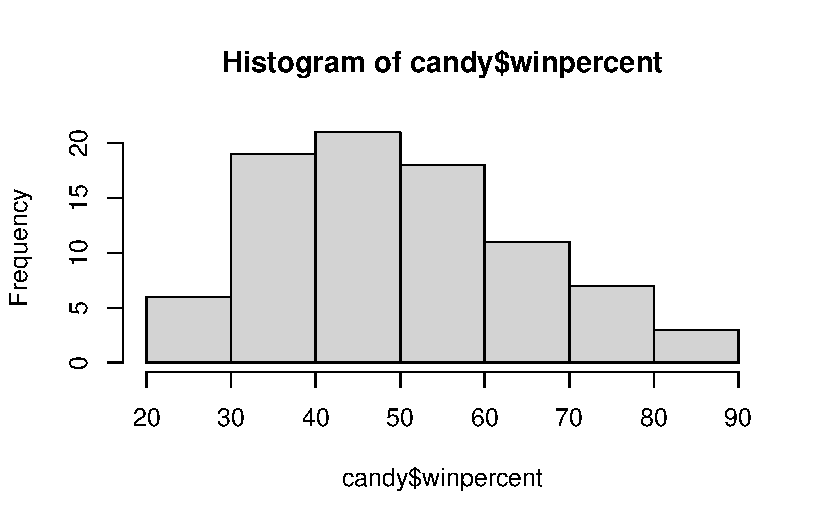
\includegraphics[keepaspectratio]{Class-9-Candy_files/figure-pdf/unnamed-chunk-8-1.pdf}}

\begin{Shaded}
\begin{Highlighting}[]
\FunctionTok{library}\NormalTok{(ggplot2)}

\FunctionTok{ggplot}\NormalTok{(candy, }\FunctionTok{aes}\NormalTok{(}\AttributeTok{x =}\NormalTok{ winpercent)) }\SpecialCharTok{+}
  \FunctionTok{geom\_histogram}\NormalTok{(}\AttributeTok{bins =} \DecValTok{20}\NormalTok{, }\AttributeTok{fill =} \StringTok{"navy"}\NormalTok{, }\AttributeTok{color =} \StringTok{"maroon"}\NormalTok{) }\SpecialCharTok{+}
  \FunctionTok{labs}\NormalTok{(}
    \AttributeTok{x =} \StringTok{"Candy Win \%"}\NormalTok{,}
    \AttributeTok{y =} \StringTok{"Frequency"}\NormalTok{,}
    \AttributeTok{title =} \StringTok{"Distribution of Candy Win Percentage"}\NormalTok{)}
\end{Highlighting}
\end{Shaded}

\pandocbounded{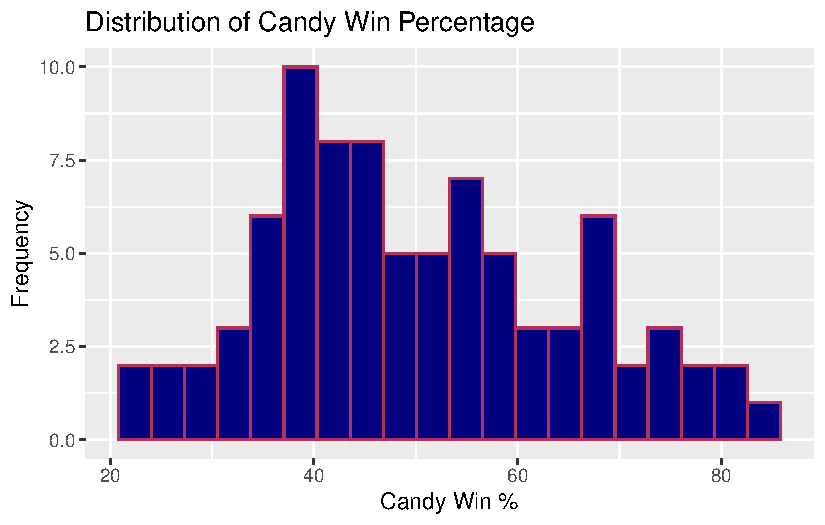
\includegraphics[keepaspectratio]{Class-9-Candy_files/figure-pdf/unnamed-chunk-9-1.pdf}}

\begin{quote}
Q9. Is the distribution of winpercent values symmetrical?
\end{quote}

The distribution of winpercent values is not symmetrical

\begin{quote}
Q10. Is the center of the distribution above or below 50\%?
\end{quote}

The center of the distribution is above 50\%

\begin{Shaded}
\begin{Highlighting}[]
\FunctionTok{mean}\NormalTok{(candy}\SpecialCharTok{$}\NormalTok{winpercent)}
\end{Highlighting}
\end{Shaded}

\begin{verbatim}
[1] 50.31676
\end{verbatim}

\begin{Shaded}
\begin{Highlighting}[]
\FunctionTok{summary}\NormalTok{(candy}\SpecialCharTok{$}\NormalTok{winpercent)}
\end{Highlighting}
\end{Shaded}

\begin{verbatim}
   Min. 1st Qu.  Median    Mean 3rd Qu.    Max. 
  22.45   39.14   47.83   50.32   59.86   84.18 
\end{verbatim}

\begin{quote}
Q11. On average is chocolate candy higher or lower ranked than fruit
candy?
\end{quote}

\begin{enumerate}
\def\labelenumi{\arabic{enumi}.}
\tightlist
\item
  Find all chocolate candy
\item
  Get their winpercent values
\item
  Find the mean
\item
  Find all fruit candy
\item
  Get their winpercent values
\item
  Find the mean
\item
  Compare the two means
\end{enumerate}

On average, chocolate candy is ranked higher than fruit candy

\begin{Shaded}
\begin{Highlighting}[]
\NormalTok{choc.candy }\OtherTok{\textless{}{-}}\NormalTok{ candy[candy}\SpecialCharTok{$}\NormalTok{chocolate }\SpecialCharTok{==} \DecValTok{1}\NormalTok{, ]}
\NormalTok{choc.win }\OtherTok{\textless{}{-}}\NormalTok{ choc.candy}\SpecialCharTok{$}\NormalTok{winpercent}
\FunctionTok{mean}\NormalTok{(choc.win)}
\end{Highlighting}
\end{Shaded}

\begin{verbatim}
[1] 60.92153
\end{verbatim}

\begin{Shaded}
\begin{Highlighting}[]
\NormalTok{fruit.candy }\OtherTok{\textless{}{-}}\NormalTok{ candy[candy}\SpecialCharTok{$}\NormalTok{fruity }\SpecialCharTok{==} \DecValTok{1}\NormalTok{, ]}
\NormalTok{fruit.win }\OtherTok{\textless{}{-}}\NormalTok{ fruit.candy}\SpecialCharTok{$}\NormalTok{winpercent}
\FunctionTok{mean}\NormalTok{(fruit.win)}
\end{Highlighting}
\end{Shaded}

\begin{verbatim}
[1] 44.11974
\end{verbatim}

\begin{quote}
Q12. Is this difference statistically significant?
\end{quote}

This difference is statistically significant

\begin{Shaded}
\begin{Highlighting}[]
\FunctionTok{t.test}\NormalTok{(choc.win, fruit.win)}
\end{Highlighting}
\end{Shaded}

\begin{verbatim}

    Welch Two Sample t-test

data:  choc.win and fruit.win
t = 6.2582, df = 68.882, p-value = 2.871e-08
alternative hypothesis: true difference in means is not equal to 0
95 percent confidence interval:
 11.44563 22.15795
sample estimates:
mean of x mean of y 
 60.92153  44.11974 
\end{verbatim}

\begin{quote}
Q13. What are the five least liked candy types in this set?
\end{quote}

\begin{Shaded}
\begin{Highlighting}[]
\FunctionTok{tail}\NormalTok{(candy[}\FunctionTok{order}\NormalTok{(candy}\SpecialCharTok{$}\NormalTok{winpercent),], }\AttributeTok{n=}\DecValTok{5}\NormalTok{)}
\end{Highlighting}
\end{Shaded}

\begin{verbatim}
                          chocolate fruity caramel peanutyalmondy nougat
Snickers                          1      0       1              1      1
Kit Kat                           1      0       0              0      0
Twix                              1      0       1              0      0
Reese's Miniatures                1      0       0              1      0
Reese's Peanut Butter cup         1      0       0              1      0
                          crispedricewafer hard bar pluribus sugarpercent
Snickers                                 0    0   1        0        0.546
Kit Kat                                  1    0   1        0        0.313
Twix                                     1    0   1        0        0.546
Reese's Miniatures                       0    0   0        0        0.034
Reese's Peanut Butter cup                0    0   0        0        0.720
                          pricepercent winpercent
Snickers                         0.651   76.67378
Kit Kat                          0.511   76.76860
Twix                             0.906   81.64291
Reese's Miniatures               0.279   81.86626
Reese's Peanut Butter cup        0.651   84.18029
\end{verbatim}

\begin{quote}
Q14. What are the top 5 all time favorite candy types out of this set?
\end{quote}

\begin{Shaded}
\begin{Highlighting}[]
\FunctionTok{head}\NormalTok{(candy[}\FunctionTok{order}\NormalTok{(candy}\SpecialCharTok{$}\NormalTok{winpercent),], }\AttributeTok{n=}\DecValTok{5}\NormalTok{)}
\end{Highlighting}
\end{Shaded}

\begin{verbatim}
                   chocolate fruity caramel peanutyalmondy nougat
Nik L Nip                  0      1       0              0      0
Boston Baked Beans         0      0       0              1      0
Chiclets                   0      1       0              0      0
Super Bubble               0      1       0              0      0
Jawbusters                 0      1       0              0      0
                   crispedricewafer hard bar pluribus sugarpercent pricepercent
Nik L Nip                         0    0   0        1        0.197        0.976
Boston Baked Beans                0    0   0        1        0.313        0.511
Chiclets                          0    0   0        1        0.046        0.325
Super Bubble                      0    0   0        0        0.162        0.116
Jawbusters                        0    1   0        1        0.093        0.511
                   winpercent
Nik L Nip            22.44534
Boston Baked Beans   23.41782
Chiclets             24.52499
Super Bubble         27.30386
Jawbusters           28.12744
\end{verbatim}

\begin{quote}
Q15. Make a first barplot of candy ranking based on winpercent values.
\end{quote}

\begin{Shaded}
\begin{Highlighting}[]
\FunctionTok{ggplot}\NormalTok{(candy) }\SpecialCharTok{+} 
  \FunctionTok{aes}\NormalTok{(winpercent, }\FunctionTok{rownames}\NormalTok{(candy)) }\SpecialCharTok{+}
  \FunctionTok{geom\_col}\NormalTok{() }\SpecialCharTok{+}
\FunctionTok{ylab}\NormalTok{(}\StringTok{""}\NormalTok{)}
\end{Highlighting}
\end{Shaded}

\pandocbounded{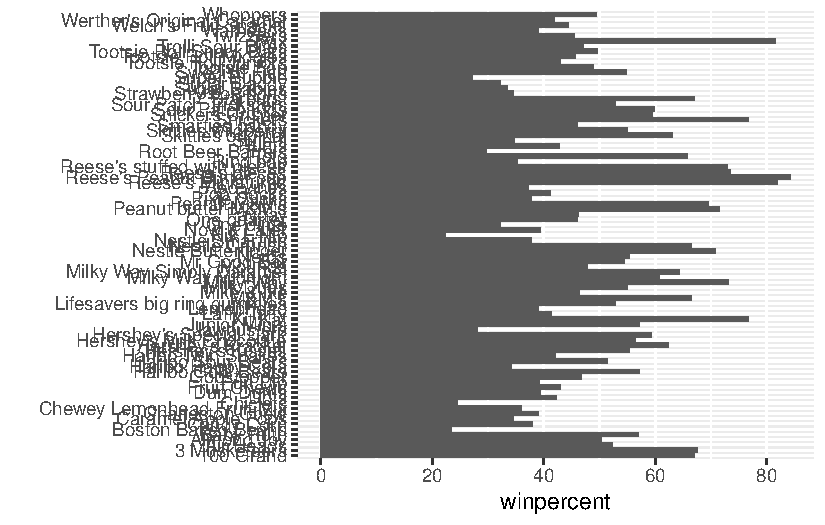
\includegraphics[keepaspectratio]{Class-9-Candy_files/figure-pdf/unnamed-chunk-17-1.pdf}}

\begin{quote}
Q16. This is quite ugly, use the reorder() function to get the bars
sorted by winpercent?
\end{quote}

\begin{Shaded}
\begin{Highlighting}[]
\FunctionTok{ggplot}\NormalTok{(candy) }\SpecialCharTok{+} 
  \FunctionTok{aes}\NormalTok{(winpercent,}
      \FunctionTok{reorder}\NormalTok{(}\FunctionTok{rownames}\NormalTok{(candy), winpercent)) }\SpecialCharTok{+}
  \FunctionTok{geom\_col}\NormalTok{() }\SpecialCharTok{+}
\FunctionTok{ylab}\NormalTok{(}\StringTok{""}\NormalTok{)}
\end{Highlighting}
\end{Shaded}

\pandocbounded{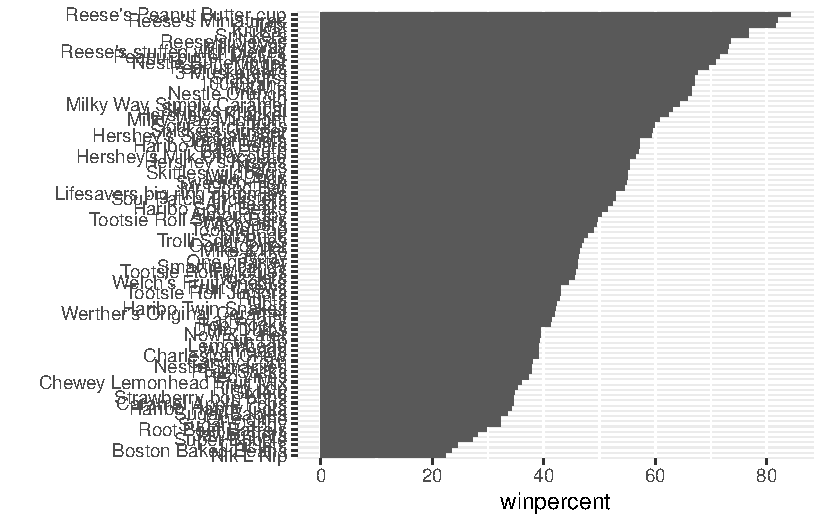
\includegraphics[keepaspectratio]{Class-9-Candy_files/figure-pdf/unnamed-chunk-18-1.pdf}}

\begin{Shaded}
\begin{Highlighting}[]
\FunctionTok{ggplot}\NormalTok{(candy) }\SpecialCharTok{+} 
  \FunctionTok{aes}\NormalTok{(winpercent,}
      \FunctionTok{reorder}\NormalTok{(}\FunctionTok{rownames}\NormalTok{(candy), winpercent),}
      \AttributeTok{fill =}\NormalTok{ chocolate) }\SpecialCharTok{+}
  \FunctionTok{geom\_col}\NormalTok{() }\SpecialCharTok{+}
\FunctionTok{ylab}\NormalTok{(}\StringTok{""}\NormalTok{)}
\end{Highlighting}
\end{Shaded}

\pandocbounded{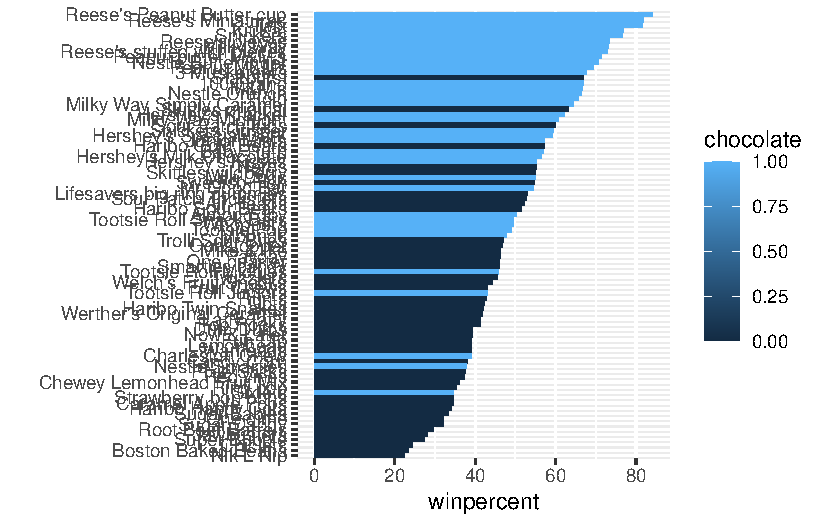
\includegraphics[keepaspectratio]{Class-9-Candy_files/figure-pdf/unnamed-chunk-19-1.pdf}}

We need a custom color vector

\begin{Shaded}
\begin{Highlighting}[]
\NormalTok{my\_cols }\OtherTok{\textless{}{-}} \FunctionTok{rep}\NormalTok{(}\StringTok{"black"}\NormalTok{, }\FunctionTok{nrow}\NormalTok{(candy))}
\NormalTok{my\_cols[candy}\SpecialCharTok{$}\NormalTok{chocolate }\SpecialCharTok{==} \DecValTok{1}\NormalTok{] }\OtherTok{\textless{}{-}}  \StringTok{"chocolate"}
\NormalTok{my\_cols[candy}\SpecialCharTok{$}\NormalTok{bar }\SpecialCharTok{==} \DecValTok{1}\NormalTok{] }\OtherTok{\textless{}{-}}  \StringTok{"brown"}
\NormalTok{my\_cols[candy}\SpecialCharTok{$}\NormalTok{fruity }\SpecialCharTok{==} \DecValTok{1}\NormalTok{] }\OtherTok{\textless{}{-}}  \StringTok{"pink"}
\NormalTok{my\_cols}
\end{Highlighting}
\end{Shaded}

\begin{verbatim}
 [1] "brown"     "brown"     "black"     "black"     "pink"      "brown"    
 [7] "brown"     "black"     "black"     "pink"      "brown"     "pink"     
[13] "pink"      "pink"      "pink"      "pink"      "pink"      "pink"     
[19] "pink"      "black"     "pink"      "pink"      "chocolate" "brown"    
[25] "brown"     "brown"     "pink"      "chocolate" "brown"     "pink"     
[31] "pink"      "pink"      "chocolate" "chocolate" "pink"      "chocolate"
[37] "brown"     "brown"     "brown"     "brown"     "brown"     "pink"     
[43] "brown"     "brown"     "pink"      "pink"      "brown"     "chocolate"
[49] "black"     "pink"      "pink"      "chocolate" "chocolate" "chocolate"
[55] "chocolate" "pink"      "chocolate" "black"     "pink"      "chocolate"
[61] "pink"      "pink"      "chocolate" "pink"      "brown"     "brown"    
[67] "pink"      "pink"      "pink"      "pink"      "black"     "black"    
[73] "pink"      "pink"      "pink"      "chocolate" "chocolate" "brown"    
[79] "pink"      "brown"     "pink"      "pink"      "pink"      "black"    
[85] "chocolate"
\end{verbatim}

\begin{Shaded}
\begin{Highlighting}[]
\FunctionTok{ggplot}\NormalTok{(candy) }\SpecialCharTok{+} 
  \FunctionTok{aes}\NormalTok{(winpercent,}
      \FunctionTok{reorder}\NormalTok{(}\FunctionTok{rownames}\NormalTok{(candy), winpercent)) }\SpecialCharTok{+}
  \FunctionTok{geom\_col}\NormalTok{(}\AttributeTok{fill =}\NormalTok{ my\_cols) }\SpecialCharTok{+}
\FunctionTok{ylab}\NormalTok{(}\StringTok{""}\NormalTok{)}
\end{Highlighting}
\end{Shaded}

\pandocbounded{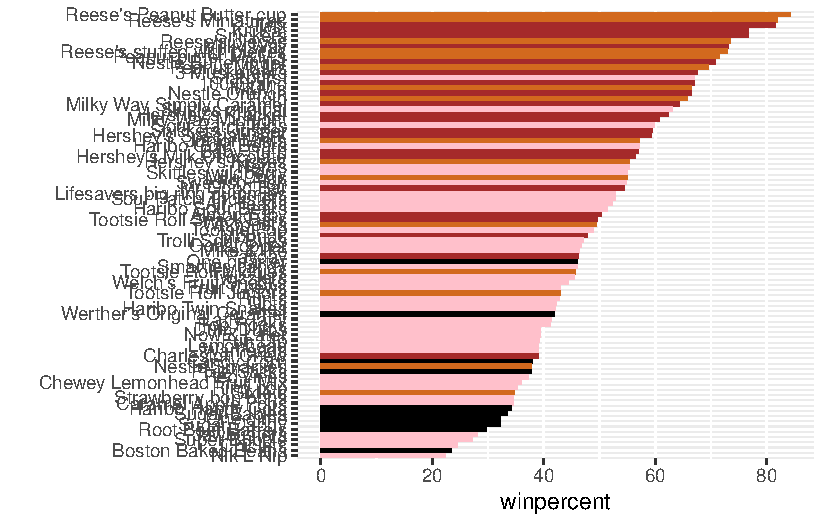
\includegraphics[keepaspectratio]{Class-9-Candy_files/figure-pdf/unnamed-chunk-21-1.pdf}}

\begin{quote}
Q17. What is the worst ranked chocolate candy?
\end{quote}

The worst ranked chocolate candy is Sixlets

\begin{Shaded}
\begin{Highlighting}[]
\FunctionTok{rownames}\NormalTok{(candy)[candy}\SpecialCharTok{$}\NormalTok{chocolate }\SpecialCharTok{==} \DecValTok{1}\NormalTok{][}\FunctionTok{which.min}\NormalTok{(candy}\SpecialCharTok{$}\NormalTok{winpercent[candy}\SpecialCharTok{$}\NormalTok{chocolate }\SpecialCharTok{==} \DecValTok{1}\NormalTok{])]}
\end{Highlighting}
\end{Shaded}

\begin{verbatim}
[1] "Sixlets"
\end{verbatim}

\begin{quote}
Q18. What is the best ranked fruity candy?
\end{quote}

The best ranked fruity candy is Starburst

\begin{Shaded}
\begin{Highlighting}[]
\FunctionTok{rownames}\NormalTok{(candy)[candy}\SpecialCharTok{$}\NormalTok{fruity }\SpecialCharTok{==} \DecValTok{1}\NormalTok{][}\FunctionTok{which.max}\NormalTok{(candy}\SpecialCharTok{$}\NormalTok{winpercent[candy}\SpecialCharTok{$}\NormalTok{fruity }\SpecialCharTok{==} \DecValTok{1}\NormalTok{])]}
\end{Highlighting}
\end{Shaded}

\begin{verbatim}
[1] "Starburst"
\end{verbatim}

\begin{Shaded}
\begin{Highlighting}[]
\FunctionTok{library}\NormalTok{(ggrepel)}

\NormalTok{my\_cols[candy}\SpecialCharTok{$}\NormalTok{fruity }\SpecialCharTok{==} \DecValTok{1}\NormalTok{] }\OtherTok{\textless{}{-}} \StringTok{"red"}

\CommentTok{\# How about a plot of win vs price}
\FunctionTok{ggplot}\NormalTok{(candy) }\SpecialCharTok{+}
  \FunctionTok{aes}\NormalTok{(winpercent, pricepercent, }\AttributeTok{label=}\FunctionTok{rownames}\NormalTok{(candy)) }\SpecialCharTok{+}
  \FunctionTok{geom\_point}\NormalTok{(}\AttributeTok{col=}\NormalTok{my\_cols) }\SpecialCharTok{+} 
  \FunctionTok{geom\_text\_repel}\NormalTok{(}\AttributeTok{col=}\NormalTok{my\_cols, }\AttributeTok{size=}\FloatTok{3.3}\NormalTok{, }\AttributeTok{max.overlaps =} \DecValTok{17}\NormalTok{)}
\end{Highlighting}
\end{Shaded}

\begin{verbatim}
Warning: ggrepel: 4 unlabeled data points (too many overlaps). Consider
increasing max.overlaps
\end{verbatim}

\pandocbounded{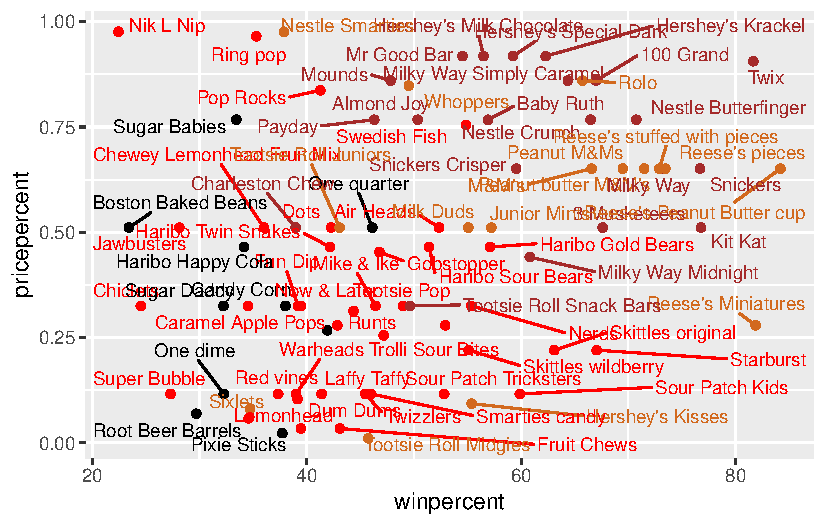
\includegraphics[keepaspectratio]{Class-9-Candy_files/figure-pdf/unnamed-chunk-24-1.pdf}}

\begin{quote}
Q19. Which candy type is the highest ranked in terms of winpercent for
the least money - i.e.~offers the most bang for your buck?
\end{quote}

The candy that's highest ranked in terms of winpercent for the least
money is chocolate candy

\begin{Shaded}
\begin{Highlighting}[]
\NormalTok{min\_price }\OtherTok{\textless{}{-}} \FunctionTok{min}\NormalTok{(candy}\SpecialCharTok{$}\NormalTok{pricepercent)}

\NormalTok{cheap\_candies }\OtherTok{\textless{}{-}}\NormalTok{ candy[candy}\SpecialCharTok{$}\NormalTok{pricepercent }\SpecialCharTok{==}\NormalTok{ min\_price, ]}

\NormalTok{best\_row }\OtherTok{\textless{}{-}} \FunctionTok{which.max}\NormalTok{(cheap\_candies}\SpecialCharTok{$}\NormalTok{winpercent)}

\FunctionTok{colnames}\NormalTok{(cheap\_candies)[best\_row]}
\end{Highlighting}
\end{Shaded}

\begin{verbatim}
[1] "chocolate"
\end{verbatim}

\begin{quote}
Q20. What are the top 5 most expensive candy types in the dataset and of
these which is the least popular?
\end{quote}

The top 5 most expensive candy types in the dataset are as follows:

\begin{Shaded}
\begin{Highlighting}[]
\NormalTok{ord }\OtherTok{\textless{}{-}} \FunctionTok{order}\NormalTok{(candy}\SpecialCharTok{$}\NormalTok{pricepercent, }\AttributeTok{decreasing =} \ConstantTok{TRUE}\NormalTok{)}
\FunctionTok{head}\NormalTok{(candy[ord,}\FunctionTok{c}\NormalTok{(}\DecValTok{11}\NormalTok{,}\DecValTok{12}\NormalTok{)], }\AttributeTok{n=}\DecValTok{5}\NormalTok{)}
\end{Highlighting}
\end{Shaded}

\begin{verbatim}
                         pricepercent winpercent
Nik L Nip                       0.976   22.44534
Nestle Smarties                 0.976   37.88719
Ring pop                        0.965   35.29076
Hershey's Krackel               0.918   62.28448
Hershey's Milk Chocolate        0.918   56.49050
\end{verbatim}

\begin{quote}
Q21. Make a barplot again with geom\_col() this time using pricepercent
and then improve this step by step, first ordering the x-axis by value
and finally making a so called ``dot chat'' or ``lollipop'' chart by
swapping geom\_col() for geom\_point() + geom\_segment().
\end{quote}

\begin{Shaded}
\begin{Highlighting}[]
\FunctionTok{ggplot}\NormalTok{(candy,}
       \FunctionTok{aes}\NormalTok{(}\AttributeTok{x =} \FunctionTok{reorder}\NormalTok{(}\FunctionTok{rownames}\NormalTok{(candy), pricepercent),}
           \AttributeTok{y =}\NormalTok{ pricepercent)) }\SpecialCharTok{+}
  \FunctionTok{geom\_col}\NormalTok{() }\SpecialCharTok{+}
  \FunctionTok{coord\_flip}\NormalTok{() }\SpecialCharTok{+}
  \FunctionTok{labs}\NormalTok{(}\AttributeTok{x =} \StringTok{"Candy"}\NormalTok{, }\AttributeTok{y =} \StringTok{"Price percent"}\NormalTok{)}
\end{Highlighting}
\end{Shaded}

\pandocbounded{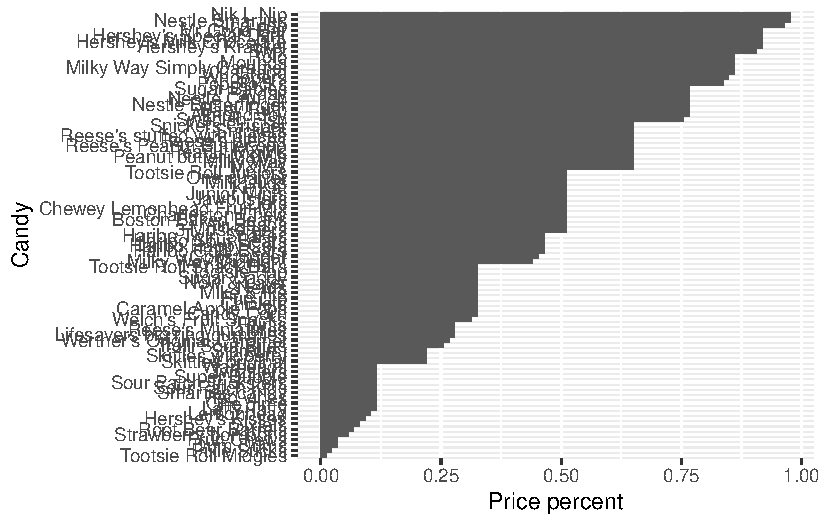
\includegraphics[keepaspectratio]{Class-9-Candy_files/figure-pdf/unnamed-chunk-27-1.pdf}}

\begin{Shaded}
\begin{Highlighting}[]
\FunctionTok{ggplot}\NormalTok{(candy) }\SpecialCharTok{+}
  \FunctionTok{aes}\NormalTok{(pricepercent, }\FunctionTok{reorder}\NormalTok{(}\FunctionTok{rownames}\NormalTok{(candy), pricepercent)) }\SpecialCharTok{+}
  \FunctionTok{geom\_segment}\NormalTok{(}\FunctionTok{aes}\NormalTok{(}\AttributeTok{yend =} \FunctionTok{reorder}\NormalTok{(}\FunctionTok{rownames}\NormalTok{(candy), pricepercent), }
                   \AttributeTok{xend =} \DecValTok{0}\NormalTok{), }\AttributeTok{col=}\StringTok{"gray40"}\NormalTok{) }\SpecialCharTok{+}
    \FunctionTok{geom\_point}\NormalTok{()}
\end{Highlighting}
\end{Shaded}

\pandocbounded{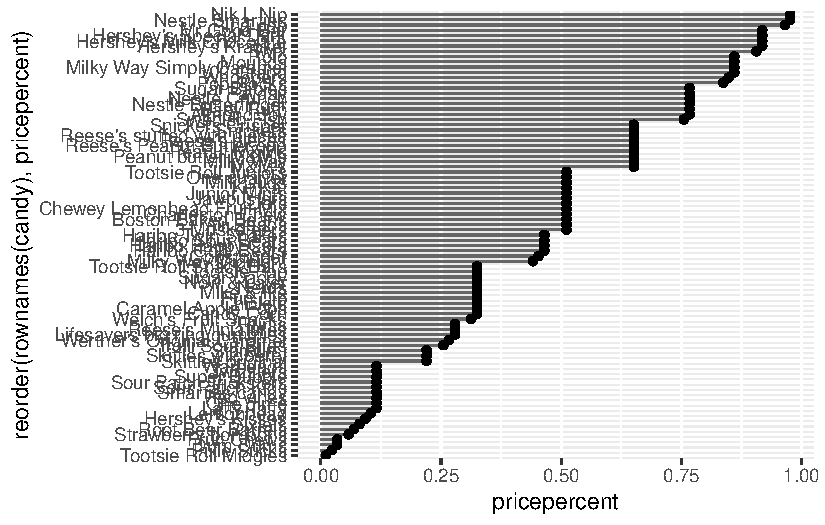
\includegraphics[keepaspectratio]{Class-9-Candy_files/figure-pdf/unnamed-chunk-28-1.pdf}}

\subsection{Exploring the Correlation
Structure}\label{exploring-the-correlation-structure}

\begin{Shaded}
\begin{Highlighting}[]
\NormalTok{cij }\OtherTok{\textless{}{-}} \FunctionTok{cor}\NormalTok{(candy)}
\end{Highlighting}
\end{Shaded}

\begin{Shaded}
\begin{Highlighting}[]
\FunctionTok{library}\NormalTok{(corrplot)}
\end{Highlighting}
\end{Shaded}

\begin{verbatim}
corrplot 0.95 loaded
\end{verbatim}

\begin{Shaded}
\begin{Highlighting}[]
\FunctionTok{corrplot}\NormalTok{(cij)}
\end{Highlighting}
\end{Shaded}

\pandocbounded{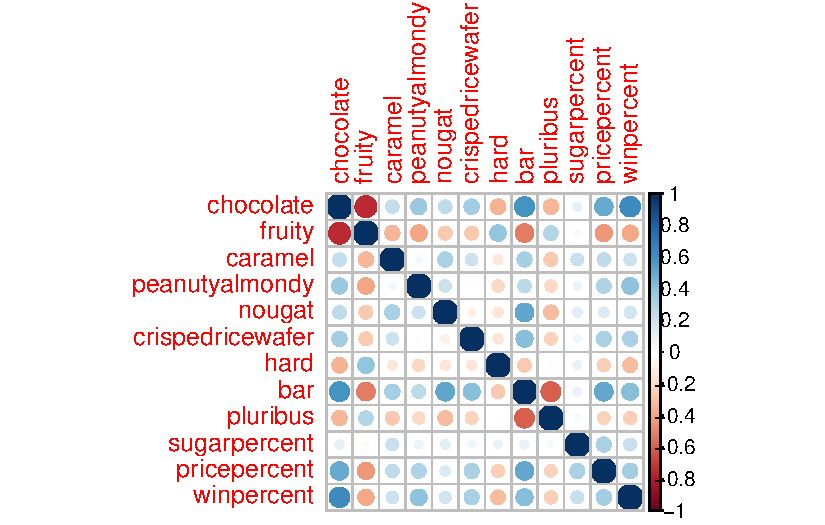
\includegraphics[keepaspectratio]{Class-9-Candy_files/figure-pdf/unnamed-chunk-30-1.pdf}}

\begin{quote}
Q22. Examining this plot what two variables are anti-correlated
(i.e.~have minus values)?
\end{quote}

The 2 variables that are anti-correlated are chocolate and fruity.

\begin{quote}
Q23. Similarly, what two variables are most positively correlated?
\end{quote}

The 2 variables that are most positively correlated are chocolate and
bar.

\subsection{Principal Component Analysis
(PCA)}\label{principal-component-analysis-pca}

\begin{Shaded}
\begin{Highlighting}[]
\NormalTok{candy2 }\OtherTok{\textless{}{-}} \FunctionTok{read.csv}\NormalTok{(}\StringTok{"https://raw.githubusercontent.com/fivethirtyeight/data/master/candy{-}power{-}ranking/candy{-}data.csv"}\NormalTok{, }\AttributeTok{row.name =} \DecValTok{1}\NormalTok{)}

\NormalTok{pca }\OtherTok{\textless{}{-}} \FunctionTok{prcomp}\NormalTok{(candy2, }\AttributeTok{scale =} \ConstantTok{TRUE}\NormalTok{)}
\FunctionTok{summary}\NormalTok{(pca)}
\end{Highlighting}
\end{Shaded}

\begin{verbatim}
Importance of components:
                          PC1    PC2    PC3     PC4    PC5     PC6     PC7
Standard deviation     2.0788 1.1378 1.1092 1.07533 0.9518 0.81923 0.81530
Proportion of Variance 0.3601 0.1079 0.1025 0.09636 0.0755 0.05593 0.05539
Cumulative Proportion  0.3601 0.4680 0.5705 0.66688 0.7424 0.79830 0.85369
                           PC8     PC9    PC10    PC11    PC12
Standard deviation     0.74530 0.67824 0.62349 0.43974 0.39760
Proportion of Variance 0.04629 0.03833 0.03239 0.01611 0.01317
Cumulative Proportion  0.89998 0.93832 0.97071 0.98683 1.00000
\end{verbatim}

Score Plot\ldots{}

\begin{Shaded}
\begin{Highlighting}[]
\FunctionTok{ggplot}\NormalTok{(pca}\SpecialCharTok{$}\NormalTok{x) }\SpecialCharTok{+}
  \FunctionTok{aes}\NormalTok{(PC1, PC2, }\AttributeTok{label =} \FunctionTok{row.names}\NormalTok{(pca}\SpecialCharTok{$}\NormalTok{x)) }\SpecialCharTok{+}
  \FunctionTok{geom\_point}\NormalTok{(}\AttributeTok{col =}\NormalTok{ my\_cols) }\SpecialCharTok{+}
\FunctionTok{geom\_text\_repel}\NormalTok{(}\AttributeTok{max.overlaps =} \DecValTok{30}\NormalTok{, }\AttributeTok{size =} \FloatTok{3.3}\NormalTok{, }\AttributeTok{col =}\NormalTok{ my\_cols) }\SpecialCharTok{+}
  \FunctionTok{theme}\NormalTok{(}\AttributeTok{legend.position =} \StringTok{"none"}\NormalTok{) }\SpecialCharTok{+}
  \FunctionTok{labs}\NormalTok{(}\AttributeTok{title=}\StringTok{"Halloween Candy PCA Space"}\NormalTok{,}
       \AttributeTok{subtitle=}\StringTok{"Colored by type: chocolate bar (dark brown), chocolate other (light brown), fruity (pink), other (black)"}\NormalTok{)}
\end{Highlighting}
\end{Shaded}

\begin{verbatim}
Warning: ggrepel: 4 unlabeled data points (too many overlaps). Consider
increasing max.overlaps
\end{verbatim}

\pandocbounded{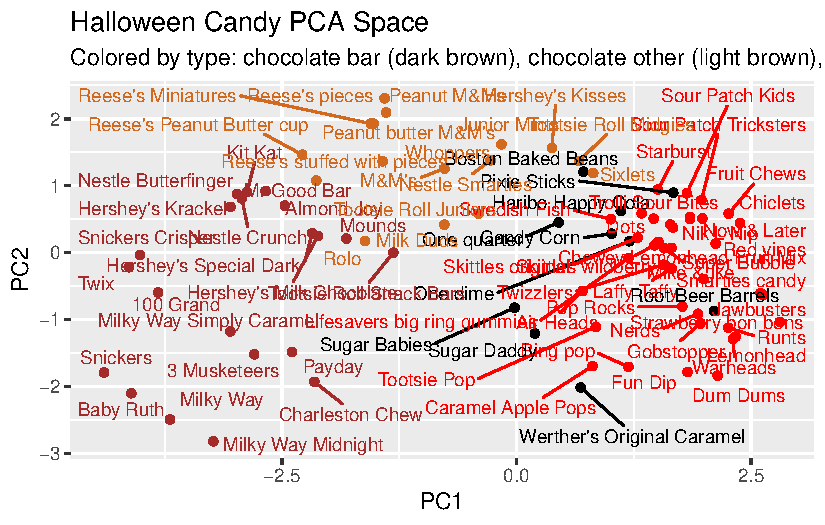
\includegraphics[keepaspectratio]{Class-9-Candy_files/figure-pdf/unnamed-chunk-32-1.pdf}}

\begin{Shaded}
\begin{Highlighting}[]
\FunctionTok{ggplot}\NormalTok{(pca}\SpecialCharTok{$}\NormalTok{rotation) }\SpecialCharTok{+}
  \FunctionTok{aes}\NormalTok{(PC1,}
    \AttributeTok{y =} \FunctionTok{reorder}\NormalTok{(}\FunctionTok{row.names}\NormalTok{(pca}\SpecialCharTok{$}\NormalTok{rotation), PC1), }\AttributeTok{x =}\NormalTok{ PC1) }\SpecialCharTok{+}
  \FunctionTok{geom\_col}\NormalTok{()}
\end{Highlighting}
\end{Shaded}

\pandocbounded{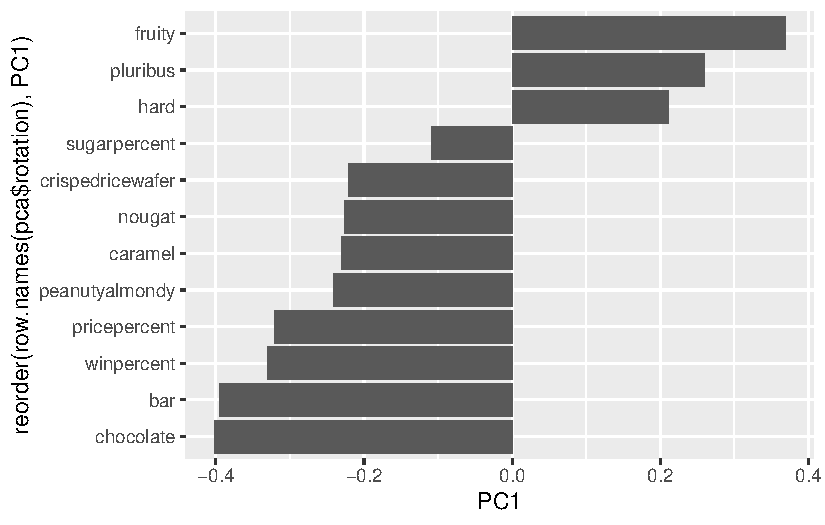
\includegraphics[keepaspectratio]{Class-9-Candy_files/figure-pdf/unnamed-chunk-33-1.pdf}}

\begin{quote}
Q24. Complete the code to generate the loadings plot above. What
original variables are picked up strongly by PC1 in the positive
direction? Do these make sense to you? Where did you see this
relationship highlighted previously?
\end{quote}

The variables that are picked up strongly by PC1 in the positive
direction are ``fruity'', ``pluribus'', and ``hard''. Yes, this does
make sense. PC1 separates the fruity, hard, sugary, and non-chocolate
candies from the chocolate candies. The positive loadings are hard,
fruit candies, whereas the negative loadings describe chocolate bars
(e.g.~chocolate, bar, caramel, nougat, etc.). This relationship was
previously highlighted in the correlation structure where chocolate and
fruity were the most anti-correlated pair. Hard candies also tended to
be non-chocolate, which was denoted by PC1. This was also evident in the
PCA scatter plot where fruity candies were clustered on one side of PC1
and chocolate was clustered on the opposite side. PC1 visually separates
the candy types in the same way the loading plots above explain
numerically.

\begin{quote}
Q25. Based on your exploratory analysis, correlation findings, and PCA
results, what combination of characteristics appears to make a
``winning'' candy? How do these different analyses (visualization,
correlation, PCA) support or complement each other in reaching this
conclusion?
\end{quote}

To make a ``winning'' candy, it must be chocolate-based, include
caramel, nougat, or nuts, and come bar-shaped. They are not fruity,
hard, or pluribus, and skew slightly higher in pricepercent. Exploratory
plots showed that these candies (e.g.~chocolate bars) were more likely
to be clustered at the top of winpercent, whereas fruity/hard candies
were clustered farther away. The correlation matrix revealed strong
positive correlations between chocolate, bar, caramel, and
peanutyalmondy traits, and a strong negative correlation with fruity and
hard candies. PCA loadings grouped chocolate, bar, caramel, nougat, and
nuts on the opposite side of fruity/hard candies. This indicates that
through visualization, correlation, and PCA analyses, chocolate bar with
caramel/nougat/nuts with a slightly premium price makes a ``winning''
candy.




\end{document}
